\chapterimage{./Pictures/cover-shell} % Chapter heading image
\chapter{TP1+TP2 : Shell}

\section{Manipulations de l’environnement et des fichiers sous UNIX}

\subsection{Exercice 1 : Découverte de quelques commandes d'archivage}
\textit{L'objectif de cet exercice est de découvrir et manipuler les commandes de téléchargement, d'archivage, de compression et de décompression de fichier}

\paragraph{1. Récupération et décompression d'une archive}
La commande \mintinline{shell}{wget <url>} permet de télécharger un fichier présent à cette adresse. Ici nous récupérons une archive que nous pouvons manipuler avec \texttt{tar}. \texttt{tar} a trois options intéréssante :
\begin{itemize}
\item L'option \texttt{-x} permet de restaurer les fichiers contenus dans une archive.
\item L'option \texttt{-c} permet de créer une nouvelle archive.
\item L'option \texttt{-f} permet d'utilise le fichier archive F ou le périphérique F (par défaut /dev/rmt0).
\end{itemize}
On découvre que l'archive télécharger contient 9 fichiers.

\paragraph{2. Manipulation de fichiers}
\begin{itemize}
\item La commande \mintinline{shell}{file <filename>} nous permet de savoir le format d'un fichier.
\item La commande \mintinline{shell}{mv <filename> <filename2>} me permet de déplacer mais aussi de renommer un "fichier1" en "fichier2". Ici j'ai utilisé la commande suivante : \texttt{mv image4.jpg image4.jpg2} .
\item La commande \mintinline{shell}{ls -lh <filename>} permet d'afficher les informations plus détaillé lisible par l'humain. Ici la commande nous apprend que le fichier \texttt{script.txt} fait 170Ko.
\item La commande \mintinline{shell}{gzip <filename>} permet de compresser un fichier. Ici le fichier \texttt{script.txt} a été compressé. Il fait maintenant  65Ko. La compréssion est donc d'environ 38.235\%.
\item La commande \mintinline{shell}{gunzip <filename>} permet de décompresser un fichier. Ici le fichier \texttt{script.txt} fait maintenant 170Ko, qui est bien la taille initial du fichier.
\end{itemize}

\paragraph{3. Création d'une nouvelle archive}
\begin{itemize}
\item La commande \mintinline{shell}{tar} permet de créer une archive sans la compresser. On peut tout de même utiliser \texttt{tar} pour archiver puis compresser des fichiers
\item La commande \mintinline{shell}{tar -z} permet de comprésser l'archive au format \texttt{gzip}.
\item La commande \mintinline{shell}{tar -cz *.jpg *.txt *.jp2} n'est pas exécutée car il est impossible d’écrire des données compressées dans le terminal. Pour sela il faut rajouter l'option \texttt{-f}.
\item La commande \mintinline{shell}{tar -cz *.jpg *.txt *.jp2 > nouvelleArchive3.tar.gz} redirige bien le résultat dans un fichier. En effet le symbole \texttt{>} permet de rediriger la sortie vers un fichier.
symbole >.
\end{itemize}
La redirection du flux dans un fichier recréer une archive compréssé "archive3" similaire à "archive2"  créé.
En conclusion l'archive 2 et 3 donne le même résultat et sont plus petit que l'archive 1 puisqu'elles sont compréssés.

\subsection{Exercice 2 : Utilisation des masques de création de fichiers}
\textit{Cet exercice permet de comprendre les droits UNIX à la création de fichier à l'aide des masque utilisateur.}
La commande \mintinline{shell}{umask} permet de définir les permissions par défaut de fichiers ou de répertoires  créees. Pour sela il faut préciser les droits que l'on veut supprimer.
Ci-dessous un tableau de droits UNIX pour rappel.

\begin{figure}[!h]
\centering
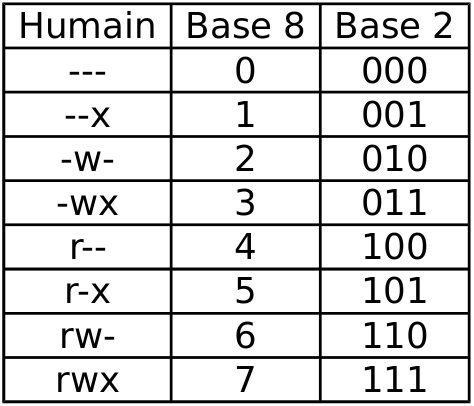
\includegraphics[width=200pt]{./shell/Pictures/permissions}
\caption{Permissions Unix}
\label{Permissions Unix}
\end{figure}

\paragraph{1.}
Afin de créer des fichiers avec les droits adecquates, il faudra effectuer les commandes suivantes :
\begin{minted}{shell}
touch Raphael.txt
umask 0666
touch Donatello.txt
umask 0331
touch Michelangelo.txt
umask 0661
touch Leonardo.txt
umask 0000
\end{minted}

\paragraph{2. et 3.}
Après plusieurs test, on découvre qu'il n'est pas possible de donner plus de droit que la limitation par défaut du systeme.
\begin{itemize}
\item \mintinline{shell}{umask 666} sur les fichiers
\item \mintinline{shell}{umask 777} sur les répertoires
\end{itemize}

\subsection{Exercice 3 : Manipulation du Systeme de fichier et des droits de navigation}
\textit{L'objectif de cet exercice est de manipuler les commandes de navigation dans l'arborescence et de création de fichier.}
\begin{itemize}
\item La commande \mintinline{shell}{mkdir <dirname>} permet de créer un répertoire.
\end{itemize}

\paragraph{1.}
L'archive contient 5 images.

\paragraph{3.}
Le chemin absolue d'un fichier ou d'un repertoire correspond au chemin vers le fichier ou repertoire depuis la racine.
Par exemple : \texttt{/home/axel/Documents/Shell/TPs/TP1/Ex3/images/Chinpokomon/P-Z/Vamporc.png}

\paragraph{4.}
Le chemin relatif d'un fichier ou d'un repertoire correspond au chemin vers le fichier ou repertoire par rapport à un autre repertoire.
Par exemple : \texttt{../P-Z/Vamporc.png}

\paragraph{6.}
La commande \mintinline{shell}{tar -xczf ITC313_TP_Shell_lebot.axel.tar.gz} permettra de décompresser et extraire l'archive.

\paragraph{7.}
Après transfert de l'archive compressé toutes les permissions sont conservés.

\subsection{Exercice 4 : Manipulation d'expression régulière}
\textit{L'objectif de cet exercice est de manipuler les basiques des expressions régulière.}

\paragraph{1.}
La commande \mintinline{shell}{wget https://cloud.infotro.fr/ITC313/unGrosBordel.txt} permettra de récupérer le fichier à analyser.

\paragraph{2.}
Les lignes affichées par \mintinline{shell}{cat unGrosBordel.txt | grep -E "ette"} contiennent toutes la suite de lettres "ette".

\paragraph{3.}
Les lignes affichées par \mintinline{shell}{cat unGrosBordel.txt | grep -E "T"} contiennent toutes la lettre "T".

\paragraph{4.}
Les lignes affichées par \mintinline{shell}{cat unGrosBordel.txt | grep -E "ˆT"} contiennent toutes la lettre "T" en début de ligne.

\paragraph{5.}
L'expression \texttt{\^} signifie donc "début".

\paragraph{6.}
Les lignes affichées par \mintinline{shell}{cat unGrosBordel.txt | grep -E "te$"} contiennent toutes la suite de lettres "te" en fin de ligne.

\paragraph{7.}
Les lignes affichées par \mintinline{shell}{cat unGrosBordel.txt | grep -E "c.r"} contiennent toutes la suite de lettres "c", un caractère quelconque, "r".

\paragraph{8.}
Les lignes affichées par \mintinline{shell}{cat unGrosBordel.txt | grep -E "(oui|non)"} contiennent toutes soit "oui", soit "non".

\paragraph{9.}
\begin{itemize}
\item \texttt{\$} représante la fin d'une ligne.
\item \texttt{|} représante une condition "ou".
\item \texttt{.} représante un caractère quelconque.
\end{itemize}

\paragraph{10.}
L'option \texttt{-o} dans la commande \mintinline{shell}{cat unGrosBordel.txt | grep -o -E "c.r"} permet de n’afficher que la partie de la ligne correspondant à l’expression "c.r" appelé "motif".

\paragraph{11.}
Les motifs affichées par \mintinline{shell}{cat unGrosBordel.txt | grep -o -E "[A-Z]"} contiennent une suite de 4 lettres majuscule.

\paragraph{12.}
Les motifs affichées par \mintinline{shell}{cat unGrosBordel.txt | grep -o -E "[A-Z][a-z]+"} contiennent une suite d'au moins une majuscule et une minuscule.

\paragraph{13.}
Les motifs affichées par \mintinline{shell}{cat unGrosBordel.txt | grep -o -E "[A-Z][a-z]*"} contiennent une suite de 0, 1 ou plus de une majuscule et une minuscule.

\paragraph{14.}
\begin{itemize}
\item \texttt{+} représante 1 ou plusieurs.
\item \texttt{*} représante 0, 1 ou plusieurs.
\end{itemize}

\paragraph{15.}
La commande
\begin{minted}{shell}
cat unGrosBordel.txt | grep -o -E "[A-Za-z0-9\.\_]+@([A-Za-z0-9\-]+\.)*[a-zA-Z]{2,4}"
\end{minted}
permet de récupérer les addresse e-mail.

\paragraph{16.}
La commande
\begin{minted}{shell}
cat unGrosBordel.txt | grep -o -E "(\+33|0)(\.| )?[0-9]((\.| )?[0-9]{2}){4}"
\end{minted}
permet de récupérer les numéro de téléphone.

\paragraph{17.}
La commande \mintinline{shell}{cat unGrosBordel.txt | grep -o -E "\(\([a-z]+\)\)"} permet de trouver la phrase secrète : "bien joue  tu as trouve la reponse a la derniere question"

\section{Éditions de scripts}

\subsection{Exercice 5 : Un premier script}
\textit{L'objectif de cet exercice est de créer un scripts basique et de l'éxécuter.}
\inputminted{bash}{../sources/shell/TP1-2/ex5.sh}

\subsection{Exercice 6 : Comptage des paramètres}
\textit{Nous verrons ici comment le passage de paramètres, le comptage et la récupération des paramètres dans un script.}
\inputminted{bash}{../sources/shell/TP1-2/ex6-parametres.sh}
La commande \texttt{shift} permet de décaler la liste d’arguments. Nous l'utiliserons dans le script suivant.
\inputminted{bash}{../sources/shell/TP1-2/ex6-parametres2.sh}

\subsection{Exercice 7 : Portée des variables}
\textit{L'exercice suivant permettra de comprendre la portée de variable et de modifications entre shell.}

\paragraph{1. Portée des variables locales}
Après avoir créé initialisé une variables midichloriens à l'aide de la commande \mintinline{shell}{midichloriens=50000}, om peut bien l'afficher avec la commande \mintinline{shell}{echo midichloriens}.
\inputminted{bash}{../sources/shell/TP1-2/ex7-yoda.sh}
On execute ensuite le script \texttt{yoda.sh} ci-dessus qui n'affiche rien. On en conclue donc que la variable initialisé dans le terminal n'est pas accessible depuis le script. \par
On essaie ensuite d'initialisé la variable \texttt{midichloriens} depuis le script \texttt{vador.sh} ci-dessous puis de ré-executer le script \texttt{yoda.sh}.
\inputminted{bash}{../sources/shell/TP1-2/ex7-vador.sh}
En éxécutant la commande \mintinline{shell}{echo midichloriens} la variable \texttt{midichloriens} reste égale à 50000. On peut donc conclure que variables sont locales à un shell ou à un script.

\paragraph{2. Portée limitée au shell}
En utilisant un second terminal, lorsque l’on affiche la valeur de la variable \texttt{midichloriens} en utilisant \mintinline{shell}{echo midichloriens}, on constate que rien ne s’affiche. \par
En lancant un sous-shell avec la commande \mintinline{shell}{bash} et en affichant la valeur de la variable \texttt{midichloriens}, rien ne s’affiche. \par
Après être sorti du sous-shell, on peut afficher la variable \texttt{midichloriens}, la valeur est toujours égale à 50000.

\paragraph{3. Étendre la portée de la valeur d’une variable locale}
En ayant éxécuté la commande \mintinline{shell}{export midichloriens} et refait les manipulations de {2.}, cette fois, la variable \texttt{midichloriens} est lisible par le sous-shell. \par
On initialise cette fois ci une variable \texttt{force} à 100. On modifie depuis le sous-shell cette valeur à 150. En fermant le sous-shell puis et en affichant la variable avec la commande \mintinline{shell}{echo force}, on s'appercoit que la variable n'a pas été modifié. \par
La commande \mintinline{shell}{export} permet d'exporter le clone d'une variable ayant le même comportement, le même nom, la même valeur.
